\chapter{वैश्विक परिवर्तन और जीवमंडल}\label{ch:b2:global-change}

1851 और 1858 के बीच हेनरी थोरो कॉनकॉर्ड, मैसाचुसेट्स के आसपास के
वनों तथा मैदानों में घूमे, और उन्होंने वह दिन लिख लिया जिस दिन कोई
पाँच सौ पौधों में से हर एक पहली बार फूला। डेढ़ सदी बाद
वनस्पतिशास्त्री उनकी नोटबुकें लेकर उन्हीं जगहों पर लौटे। जिस
ऊँची झाड़ी वाली ब्लूबेरी को थोरो ने 11 मई को खुलते देखा वह अब
12 अप्रैल को खुलती है; पूरा वनस्पति-समूह उनके समय से औसतन दस दिन पहले
फूलता है, यानी ऐसे वसंत के साथ क़दम मिलाकर जो \qty{2.4}{\celsius}
गरम है; और उनकी एक चौथाई जातियाँ कॉनकॉर्ड से जा चुकी हैं --- और वह भी
यादृच्छिक रूप से नहीं, बल्कि वे जिनका पुष्पन उस
ताप के पीछे नहीं चल सका। पिछले अध्यायों ने वह मशीनरी दी:
\cref{ch:b2:biogeochemical-cycles} के चक्र,
\cref{ch:b2:population-genetics} का वरण तथा अपवाह,
\cref{ch:b2:speciation} की होड़ तथा जाति-उद्भव, और \cref{ch:b2:living-soil} की मिट्टियाँ।
यह अध्याय उस पर कोई अंक रखता है जो जीवों के साथ हो रहा है
ज्यों-ज्यों कोई एक जाति वायु तथा समुद्र का रसायन बदलती है: कार्बन के प्रति टन
कितना तापन, प्रति अंश वसंत के कितने दिन, कितने मीटर ऊपर की ओर,
समुद्र में कितना अम्ल, प्रति हेक्टेयर कितनी
जातियाँ खोईं --- और वे अंक आने वाली सदी के बारे में
क्या कहते हैं।

\section{भौतिक परिवर्तन}

\begin{proposition}[तापन संचयी उत्सर्जनों के समानुपाती है]\label{prop:b2:global-change:tcre}
\index{वैश्विक तापन}\index{संचयी उत्सर्जन}\index{कार्बन बजट}\index{हरितगृह प्रभाव}
कार्बन डाइऑक्साइड उस अवरक्त को अवशोषित करती है जो वह ज़मीन उत्सर्जित करती है और उसका
एक भाग लौटा देती है; अधिक \ensuremath{\mathrm{CO_2}} का अर्थ है कोई गरम सतह, यानी
हर दुगुनाकरण पर लगभग \qty{3}{\celsius}, जब वे महासागर पकड़ लें
(यानी \emph{जलवायु संवेदिता})। चूँकि \ensuremath{\mathrm{CO_2}} के प्रति
ताप-अनुक्रिया सांद्रता में लघुगणकीय है जबकि उत्सर्जनों का \omterm{prop:b2:biogeochemical-cycles:carbon}{वायुवाहित
अंश} उस सांद्रता के चढ़ने के साथ गिरता है, इसलिए वे दोनों
वक्रताएँ लगभग कट जाती हैं, और वह वैश्विक माध्य तापन, किसी अच्छे
सन्निकटन तक, \emph{उत्सर्जित कार्बन की संचयी मात्रा में रैखिक} है,
समय जो भी हो:
\[
\Delta T \approx \lambda\,C_{\text{संचयी}}, \qquad \lambda \approx
\qty{1.65}{\celsius} \text{ प्रति } \qty{1000}{GtC}
\]
(\ensuremath{\mathrm{CO_2}} के प्रति \qty{1000}{Gt} पर \qty{0.45}{\celsius})। 1850 से
उत्सर्जित कोई \qty{700}{GtC} ने इस ग्रह को \qty{1.2}{\celsius}
गरम किया है --- और वह संबंध हर लक्ष्य को कोई
बजट देता है: \qty{1.5}{\celsius} कुल मिलाकर लगभग \qty{900}{GtC} की छूट देता है,
यानी जितना उत्सर्जित हो चुका उससे \qty{200}{GtC} अधिक, यानी वर्तमान
दर पर बीस वर्ष। वह तापन असमान है: स्थल पर औसत से दुगुना
और आर्कटिक में तिगुना; रातें दिनों से अधिक; और वह बाक़ी सब के साथ आता
है --- अधिक तीखी वर्षा तथा लंबे सूखे, वर्ष भर में \qty{4}{mm} चढ़ता
समुद्र-तल, ऐसी बर्फ़ जो ग्रीष्म में पाँचवें भाग छोटी है, और
ऐसा महासागर जिसने उस ऊष्मा का \qty{90}{\%} और उस कार्बन का
एक चौथाई सोख लिया है।
\end{proposition}
\begin{proof}[प्रमाण-सामग्री]
वह समानुपातिता हर जटिलता के जलवायु-प्रतिरूपों में मिली
और देखे गए अभिलेख से पुष्ट हुई: 1850 से हुए तापन को \omterm{prop:b2:global-change:tcre}{संचयी
उत्सर्जनों} के सापेक्ष आलेखित करने पर दशकों भर एक सीधी
रेखा मिलती है। स्वयं वह \omterm{prop:b2:global-change:tcre}{हरितगृह प्रभाव}
कक्षा से मापा जाता है: उपग्रह उस अवरक्त को देखते हैं जो पृथ्वी उत्सर्जित करती है, जिसमें से
\ensuremath{\mathrm{CO_2}}, मीथेन तथा जलवाष्प की अवशोषण-पट्टियाँ कटी हुई हैं,
और वह कटाव 1970 तथा 2020 के बीच ठीक उतना गहरा हुआ है
जितना इन गैसों की चढ़ाई बताती है। \cref{ch:b2:biogeochemical-cycles} के
समस्थानिक तथा गिरती ऑक्सीजन उस अतिरिक्त
\ensuremath{\mathrm{CO_2}} को जीवाश्म ईंधन से बाँध देते हैं।
\end{proof}

\begin{omfigure}
\begin{tikzpicture}
\begin{axis}[
  width=0.88\linewidth, height=5.6cm,
  axis x line=bottom, axis y line=left,
  xmin=1845, xmax=2030, ymin=-0.3, ymax=1.5,
  xlabel={दशक}, ylabel={1850--1900 से तापन (\unit{\celsius})},
  xlabel style={font=\small, at={(axis description cs:0.5,-0.13)}, anchor=north},
  ylabel style={font=\small},
  tick label style={font=\small}, xtick={1850,1900,1950,2000}, ytick={0,0.5,1,1.5},
  scaled x ticks=false, x tick label style={/pgf/number format/1000 sep=},
  clip=false,
]
\addplot[ybar, bar width=7pt, fill=omThm!50, draw=omThm] coordinates {
(1855,0.00) (1865,-0.04) (1875,0.02) (1885,-0.06) (1895,-0.02) (1905,-0.10) (1915,-0.06) (1925,0.05) (1935,0.15) (1945,0.25) (1955,0.15) (1965,0.15) (1975,0.18) (1985,0.40) (1995,0.55) (2005,0.78) (2015,1.02) (2023,1.28)};
\node[font=\scriptsize, anchor=west, align=left] at (axis cs:1850,1.2) {हर पट्टी: किसी दशक का माध्य; अंतिम, 2020--2024\\ \qty{700}{GtC} उत्सर्जित, $\qty{1.65}{\celsius}/\qty{1000}{GtC}$: \qty{1.2}{\celsius}};
\end{axis}
\end{tikzpicture}

{\small दशक-दर-दशक वैश्विक माध्य सतही ताप, उन्नीसवीं सदी के
उत्तरार्ध के सापेक्ष। पिछले चार दशकों में से हर एक ने
कोई कीर्तिमान बनाया, और 1970 से हुई चढ़ाई प्रति दशक \qty{0.2}{\celsius}
है।}
\end{omfigure}

\section{पंचांग: ऋतु-विज्ञान}

\begin{theorem}[अंश-दिन और वसंत का जल्दी आना]\label{thm:b2:global-change:phenology}
\index{ऋतु-विज्ञान}\index{अंश-दिन}\index{तापीय समय}\index{ऋतु-वैज्ञानिक बेमेल}
पौधों तथा बहिस्तापियों के जीवन की बहुत-सी घटनाएँ --- कलिका-स्फुटन,
पुष्पन, अंड-स्फुटन, निर्गमन --- तब होती हैं जब किसी आरंभ-तिथि से जमा
\emph{\omterm{thm:b2:global-change:phenology}{तापीय समय}}, यानी किसी आधार $T_b$ से ऊपर दैनिक
तापों का योग (यानी \emph{अंश-दिन}), किसी नियत योग $K$ तक पहुँचे।
यदि वसंत का ताप रैखिक रूप से चढ़े, $T(t) = T_b
+ b\,(t - t_0)$, प्रति दिन $b$ अंश पर, उस दिन $t_0$ से जब वह उस आधार को पार करे,
तो वह घटना तब होती है:
\[
t^{*} = t_0 + \sqrt{2K/b},
\]
और $\Delta T$ का कोई एकसमान तापन उस पार करने के दिन को
$\Delta T/b$ आगे ले आता है और उसके साथ वह घटना भी: प्रति दिन $b \approx
\qty{0.1}{\celsius}$ के साथ, \emph{प्रति अंश लगभग दस दिन
पहले}। जातियाँ $T_b$, $K$ में और इसमें भिन्न हैं कि क्या वे
दिन-लंबाई भी काम में लेती हैं, जिसे तापन बदलता नहीं --- इसलिए किसी
आहार-शृंखला के सदस्य भिन्न दरों से आगे बढ़ते हैं और उनका समय
बिखर जाता है: यानी उस इल्ली तथा उस चिड़िया के बीच कोई \emph{\omterm{thm:b2:global-change:phenology}{ऋतु-वैज्ञानिक बेमेल}}
जिसे अपने चूज़े उस पर पालने हैं।
\end{theorem}
\begin{proof}
$t_0$ से अंश-दिन: $\int_{t_0}^{t}(T - T_b)\,\mathrm{d}t' =
b\,(t - t_0)^{2}/2$, जो $K$ के बराबर है जब $t - t_0 = \sqrt{2K/b}$।
$\Delta T$ का तापन $T$ को $T + \Delta T$ से बदल देता है: वह आधार
$\Delta T/b$ दिन पहले पार होता है और वह जमाव, उस दिन से आगे एक जैसा,
$\Delta T/b$ दिन पहले पूरा होता है। (यदि वह
तापन $b$ को भी तीखा करे, तो अंतराल $\sqrt{2K/b}$ भी छोटा
हो जाता है।) दिन-लंबाई से संकेतित कोई जाति अपनी तिथि रखती है; और
अंश-दिनों से संकेतित कोई चलती है; और उनके बीच का अंतर $\Delta T/b$ से बढ़ता है।
\end{proof}
\begin{proof}[प्रमाण-सामग्री]
थोरो का कॉनकॉर्ड-वनस्पति-समूह, और नॉरफ़ोक में 1736 से 1947 तक रखा गया
मार्शम परिवार का वसंत के सत्ताईस चिह्नों का अभिलेख,
दोनों पुष्पन तथा पत्ती-निकलने को वसंत के प्रति अंश तापन पर
\qtyrange{3}{6}{d} जल्दी होते दिखाते हैं। क्योतो का चेरी-पुष्प, जो
नौवीं सदी से दरबारी दैनंदिनियों में दिनांकित है,
हज़ार वर्ष तक अप्रैल के मध्य के आसपास रहा और 1900 से अप्रैल के आरंभ में
आ गया है, और अभिलेख की सबसे जल्दी तिथियाँ 2020 के दशक में पड़ी हैं। नीदरलैंड में
बलूत की इल्लियाँ अब 1985 से दो सप्ताह पहले शिखर पाती हैं; और
बड़ी टिटहरी, जो उसी गरमाहट से संकेतित है, साथ चलती रही, पर चितकबरा
मक्खीमार, जो अफ़्रीका से अपना प्रवास दिन-लंबाई से समयबद्ध करता है,
पहले की तरह पहुँचता है और उस शिखर को गया हुआ पाता है --- और जहाँ वह बेमेल सबसे बड़ा है
वहाँ उसकी समष्टियाँ \qty{90}{\%} गिर चुकी हैं (बोथ तथा
सहयोगी, 2006)।
\end{proof}

\begin{omfigure}
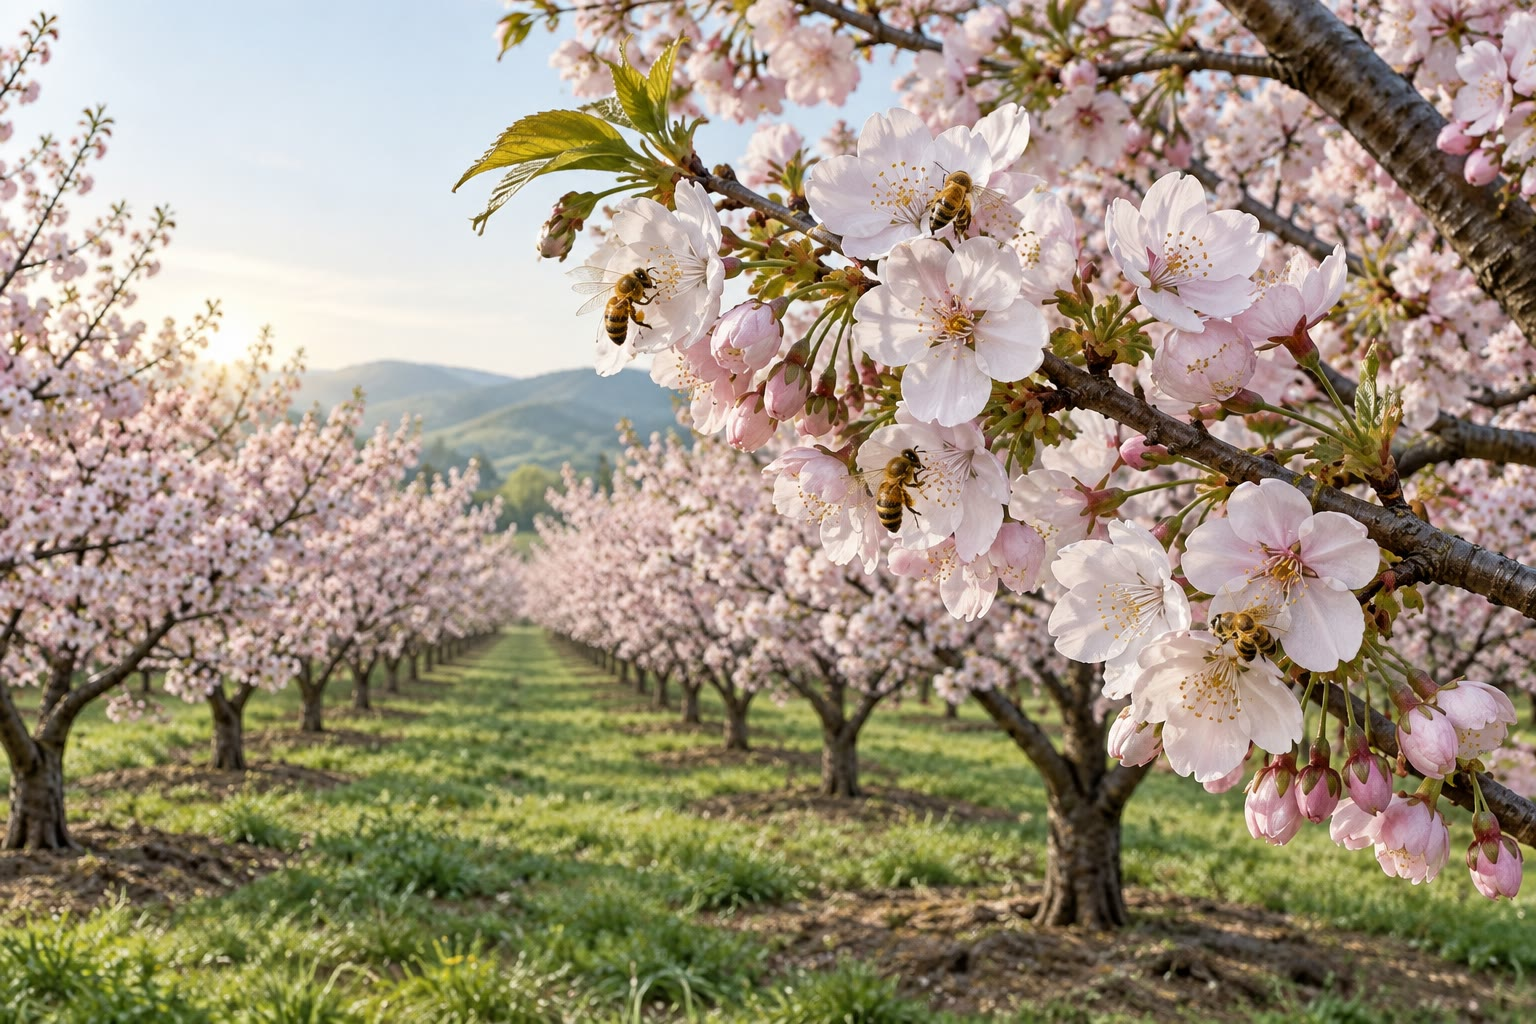
\includegraphics[width=0.62\linewidth]{images/book4/ai/b4-27-phenology-cherry.jpg}

{\small खिला हुआ कोई चेरी-बाग़। क्योतो की चेरियाँ, जो
बारह शताब्दियों तक दैनंदिनियों में दिनांकित रहीं, अब 1900 से पहले के किसी भी वर्ष से
जल्दी खुलती हैं --- और जो मधुमक्खियाँ उनका \omterm{def:b2:angiosperm-reproduction:pollination}{परागण} करती हैं उन्हें उसी दिन
उड़ते होना चाहिए।}
\end{omfigure}

\begin{omfigure}
\begin{tikzpicture}
\begin{axis}[
  width=0.74\linewidth, height=5.4cm,
  axis x line=bottom, axis y line=left,
  xmin=0, xmax=100, ymin=0, ymax=14,
  xlabel={1 मार्च से दिन}, ylabel={दैनिक माध्य ताप (\unit{\celsius})},
  xlabel style={font=\small, at={(axis description cs:0.5,-0.13)}, anchor=north},
  ylabel style={font=\small},
  tick label style={font=\small}, xtick={0,20,40,60,80,100},
  legend style={font=\scriptsize, at={(0.03,0.97)}, anchor=north west, draw=none},
  clip=false,
]
\addplot[very thick, omDef, domain=0:100, samples=2] {2 + 0.1*x};
\addlegendentry{तापन से पहले वसंत}
\addplot[very thick, omThm, domain=0:100, samples=2] {3 + 0.1*x};
\addlegendentry{\qty{1}{\celsius} गरम वसंत}
\draw[dashed, gray] (axis cs:0,5) -- (axis cs:100,5); \node[font=\scriptsize, anchor=south east] at (axis cs:100,5) {आधार ताप $T_b = \qty{5}{\celsius}$};
\fill[omDef, opacity=0.15] (axis cs:30,5) -- (axis cs:93,5) -- (axis cs:93,11.3) -- cycle;
\fill[omThm, opacity=0.15] (axis cs:20,5) -- (axis cs:83,5) -- (axis cs:83,11.3) -- cycle;
\draw[<->, thick] (axis cs:83,1.6) -- (axis cs:93,1.6); \node[font=\scriptsize, anchor=south] at (axis cs:88,1.8) {10 दिन};
\draw[dotted] (axis cs:93,0) -- (axis cs:93,5); \draw[dotted] (axis cs:83,0) -- (axis cs:83,5);
\node[font=\scriptsize, anchor=south, align=center] at (axis cs:62,11.4) {$K = 200$ अंश-दिन\\ (छायित क्षेत्रफल)};
\end{axis}
\end{tikzpicture}

{\small अंश-दिन। वह घटना तब होती है जब उस ताप-रेखा तथा उस आधार के
बीच का छायित क्षेत्रफल $K$ तक पहुँचे; और एक अंश गरम कोई वसंत
उस आधार को दस दिन पहले पार करता है तथा उस योग को
दस दिन पहले पूरा करता है।}
\end{omfigure}

\section{नक़्शा: परास-खिसक}

\begin{proposition}[समताप-रेखाएँ चलती हैं, और जातियाँ पीछे चलती हैं]\label{prop:b2:global-change:range}
\index{परास-खिसक}\index{जलवायु-वेग}\index{ह्रास दर}
समशीतोष्ण कटिबंध में ताप ऊँचाई के प्रति किलोमीटर लगभग
\qty{6.5}{\celsius} और अक्षांश के प्रति सौ किलोमीटर लगभग
\qty{0.65}{\celsius} गिरता है; इसलिए \qty{1}{\celsius} का कोई तापन
हर समताप-रेखा को लगभग \qty{150}{m} ऊपर और
\qty{150}{km} ध्रुव की ओर चला देता है। जिन जातियों की सीमाएँ ताप से बैठती हैं वे
यदि चल सकें तो अपनी समताप-रेखा के साथ चलती हैं: अध्ययन की गई सैकड़ों जातियों का
औसत 1970 से प्रति दशक \qty{11}{m} ऊपर और \qty{17}{km}
ध्रुव की ओर खिसका है, यानी उन समताप-रेखाओं की गति से, और
सबसे तेज़ --- चल, सामान्यजीवी, अल्पजीवी --- उनसे आगे निकल जाती हैं,
जबकि वृक्ष, जिनके \omterm{def:b2:angiosperm-reproduction:seed}{बीज} वर्ष भर में मीटर भर चलते हैं, और वे जातियाँ जो पहले ही
शिखर या ध्रुव पर हैं, पीछे नहीं चल सकतीं: किसी पर्वत के शीर्ष के पास
जाने को कहीं नहीं है, और तापन का हर अंश हर परास के सबसे ऊँचे
\qty{150}{m} हटा देता है। समुद्री जातियाँ, जिनके सामने कोई बाधा नहीं और जिनकी
तापीय सीमाएँ तीखी हैं, सबसे तेज़ चलती हैं, यानी प्रति दशक दसियों किलोमीटर;
कॉड, मैकरेल और उनके साथ वे मछलियाँ पूरे-पूरे समुद्रों के आरपार उत्तर
चली गई हैं। किसी परास का ऊपरी किनारा आगे बढ़ता है, और निचला
किनारा पीछे हटता है ज्यों-ज्यों वह गरम हो तथा नीचे से नए होड़ी आएँ,
और किसी भी बिंदु पर वह समुदाय ऐसी जातियों से फिर जोड़ा जाता है
जो कभी मिली ही नहीं।
\end{proposition}
\begin{proof}[प्रमाण-सामग्री]
पार्मेसन (1996) ने एडिथ के चेकरस्पॉट तितली का उसके पश्चिमी उत्तर
अमेरिकी परास भर फिर सर्वेक्षण किया: दक्षिणी किनारे तथा नीची ऊँचाइयों की
समष्टियाँ विलुप्त थीं, उत्तरी किनारे तथा ऊँची ऊँचाइयों की फल-फूल रही थीं,
और पूरा परास \qty{92}{km} उत्तर तथा \qty{124}{m} ऊपर चल चुका था ---
यानी उन समताप-रेखाओं के पीछे चलती दिखाई गई पहली जाति। ल्वानोर तथा सहयोगियों (2008) ने
फ़्रांसीसी पर्वतों भर 1905--1985 के वन-पादप सर्वेक्षणों की
1986--2005 से तुलना की: 171 जातियों की अनुकूल ऊँचाई
प्रति दशक \qty{29}{m} चढ़ चुकी थी। चेन तथा सहयोगियों (2011) ने,
दो हज़ार जातियों भर, वे खिसकें पहले के आकलनों से दो से तीन गुना तेज़
और स्थानीय तापन के समानुपाती पाईं।
\end{proof}

\begin{omfigure}
\begin{tikzpicture}[every node/.style={font=\scriptsize}, >=stealth]
  \fill[gray!25] (0,0) -- (3.5,4.2) -- (7,0) -- cycle;
  \draw[thick] (0,0) -- (3.5,4.2) -- (7,0);
  \foreach \y/\lab in {1.0/{\qty{12}{\celsius}}, 2.2/{\qty{8}{\celsius}}, 3.4/{\qty{4}{\celsius}}} { \draw[omDef, thick] ({\y/1.2},\y) -- ({7-\y/1.2},\y) node[right] {\lab}; }
  \foreach \y in {1.15,2.35,3.55} { \draw[omThm, thick, dashed] ({\y/1.2},\y) -- ({7-\y/1.2},\y); }
  \node[omThm, anchor=west, align=left] at (7.6,3.7) {बिंदुदार: \qty{1}{\celsius} तापन के बाद\\ वही समताप-रेखाएँ,\\ \qty{150}{m} ऊँची};
  \fill[omProp!50] (0.83,1.0) -- (6.17,1.0) -- (5.17,2.2) -- (1.83,2.2) -- cycle;
  \node[align=center] at (3.5,1.6) {किसी जाति की पट्टी,\\ \qtyrange{1000}{1200}{m}};
  \draw[->, thick, omExo!80!black] (1.1,2.2) -- (1.1,2.9); \node[omExo!80!black, anchor=east, align=right] at (0.95,2.55) {वह पट्टी ऊपर चलती\\ है और सिकुड़ती है};
  \node[anchor=north] at (3.5,-0.1) {कोई पर्वत: क्षेत्रफल ऊँचाई के साथ सिकुड़ता है, और उस शिखर से ऊँचा कहीं नहीं};
\end{tikzpicture}

{\small किसी पर्वत पर कोई परास-खिसक। हर अंश उन
समताप-रेखाओं को \qty{150}{m} उठाता है; कोई जाति अपनी पट्टी के पीछे ऊपर किसी
छोटे क्षेत्रफल में चलती है, और शिखर पर पहले से पड़ी कोई पट्टी खो जाती है।}
\end{omfigure}

\section{समुद्र: अम्लीकरण और ऊष्मा}

\begin{theorem}[अम्लीकरण]\label{thm:b2:global-change:acid}
\index{महासागर-अम्लीकरण}\index{कार्बोनेट तंत्र}\index{संतृप्ति अवस्था}\index{प्रवाल-विवर्णन}
समुद्री जल में घुलती कार्बन डाइऑक्साइड कार्बोनिक अम्ल बनाती है, जो
वियोजित होता है: $\ensuremath{\mathrm{CO_2}} + \ensuremath{\mathrm{H_2O}} \rightleftharpoons \ensuremath{\mathrm{H^{+}}} +
\ensuremath{\mathrm{HCO_3^{-}}}$, जिसमें $[\ensuremath{\mathrm{H^{+}}}][\ensuremath{\mathrm{HCO_3^{-}}}]/[\ensuremath{\mathrm{CO_2}}] = K_1$।
बाइकार्बोनेट उस महासागर का सबसे बड़ा कार्बन-कोष है और उस क्षारकता से लगभग
अचल थमा है, इसलिए
\[
[\ensuremath{\mathrm{H^{+}}}] \propto p_{\ensuremath{\mathrm{CO_2}}}, \qquad
\Delta\mathrm{pH} \approx -\log_{10}\frac{p_{\ensuremath{\mathrm{CO_2}}}}{p_0}
\]
--- ठीक-ठीक कहें तो उस अनुपात का $-0.9\log_{10}$, क्योंकि बाइकार्बोनेट
थोड़ा चढ़ता है। 280 से \qty{420}{ppm} तक सतही pH
$0.15$ गिर चुका है, यानी $8.2$ से $8.05$: यानी हाइड्रोजन आयनों में \qty{40}{\%} की
वृद्धि; और \qty{800}{ppm} पर वह $0.4$ गिरता। वे अतिरिक्त हाइड्रोजन
आयन कार्बोनेट खपा देते हैं, $\ensuremath{\mathrm{H^{+}}} + \ensuremath{\mathrm{CO_3^{2-}}} \to \ensuremath{\mathrm{HCO_3^{-}}}$, और
कैल्सियम कार्बोनेट की \emph{\omterm{thm:b2:global-change:acid}{संतृप्ति अवस्था}} $\Omega$ ---
यानी कैल्सियम तथा कार्बोनेट सांद्रताओं का गुणनफल बँटा वह
विलेयता-गुणनफल --- उसी अनुपात में गिरती है: ऐरागोनाइट (प्रवाल, टेरोपॉड) के
कवच तथा कंकाल $\Omega > 3$ पर सहज बनते हैं, 1 के पास
कठिनाई से, और उससे नीचे घुल जाते हैं; और वह उष्णकटिबंधीय सतह,
जो उद्योग से पहले $\Omega \approx 4$ पर थी और अब 3 पर,
\qty{560}{ppm} पर 2 तक पहुँचती है, तथा ठंडी, \ensuremath{\mathrm{CO_2}}-भरी ध्रुवीय सतही जलराशि
सबसे पहले 1 तक पहुँचती है।
\end{theorem}
\begin{proof}
उस साम्य से, $[\ensuremath{\mathrm{H^{+}}}] = K_1[\ensuremath{\mathrm{CO_2}}]/[\ensuremath{\mathrm{HCO_3^{-}}}]$ और
$[\ensuremath{\mathrm{CO_2}}]$ हेनरी के नियम से $p_{\ensuremath{\mathrm{CO_2}}}$ के समानुपाती है;
और $[\ensuremath{\mathrm{HCO_3^{-}}}]$ अचल होने पर $[\ensuremath{\mathrm{H^{+}}}]$
$p_{\ensuremath{\mathrm{CO_2}}}$ के समानुपाती है और $\mathrm{pH} = -\log_{10}[\ensuremath{\mathrm{H^{+}}}]$ उस अनुपात के
$-\log_{10}$ भर बदलता है। दूसरा साम्य, $[\ensuremath{\mathrm{H^{+}}}][\ensuremath{\mathrm{CO_3^{2-}}}]/[\ensuremath{\mathrm{HCO_3^{-}}}]
= K_2$, देता है $[\ensuremath{\mathrm{CO_3^{2-}}}] \propto 1/[\ensuremath{\mathrm{H^{+}}}] \propto
1/p_{\ensuremath{\mathrm{CO_2}}}$, इसलिए $\Omega$ गिरता है ज्यों-ज्यों $p_{\ensuremath{\mathrm{CO_2}}}$ चढ़े, और
$[\ensuremath{\mathrm{H^{+}}}]$ में \qty{40}{\%} की चढ़ाई
कार्बोनेट में \qty{30}{\%} की गिरावट है। (पूरा रसायन, बाइकार्बोनेट में परिवर्तन तथा
उन आयन-सक्रियताओं समेत, वह गुणक $0.9$ तथा वे देखे गए
अंक देता है; और वर्ष 3 का खंड उसे बरतता है।)
\end{proof}
\begin{proof}[प्रमाण-सामग्री]
हवाई के उत्तर वाला महासागर-स्टेशन 1988 से हर महीने सतही pH
मापता आया है: वह वर्ष भर में $0.0018$ गिरता है, यानी अपने ऊपर
मौना लोआ की \ensuremath{\mathrm{CO_2}} के साथ क़दम मिलाकर, जैसा वह रसायन माँगता है।
टेरोपॉड --- समुद्र के घोंघे, सामन तथा ह्वेलों का भोजन ---
प्रशांत तट से इकट्ठे किए गए अपने ऐरागोनाइट कवच
गड्ढेदार तथा घुलते हुए दिखाते हैं, वहाँ जहाँ उत्प्लवन $\Omega <
1$ वाला जल सतह पर लाता है। प्रवाल-विवर्णन ऊष्मा है, अम्ल नहीं: जब वह
जल ग्रीष्म की अधिकतम से \qty{1}{\celsius} ऊपर कुछ
सप्ताह बना रहे, तब वह प्रवाल अपने सहजीवी शैवाल निकाल देता है और भूखा मरता है; और वह ग्रेट
बैरियर रीफ़ 1998, 2002, 2016, 2017, 2020, 2022 तथा 2024 में विवर्णित हुई,
और 1995 से उसका आधा प्रवाल-आवरण जा चुका है।
\end{proof}

\begin{omfigure}
\begin{tikzpicture}
\begin{axis}[
  width=0.68\linewidth, height=5.4cm,
  axis x line=bottom, axis y line=left,
  xmin=250, xmax=1000, ymin=7.6, ymax=8.3,
  xlabel={वायुमंडलीय \ensuremath{\mathrm{CO_2}} (ppm)}, ylabel={सतही pH},
  xlabel style={font=\small, at={(axis description cs:0.5,-0.13)}, anchor=north},
  ylabel style={font=\small},
  tick label style={font=\small}, xtick={280,420,560,800,1000}, ytick={7.6,7.8,8.0,8.2},
  clip=false,
]
\addplot[very thick, omDef, domain=250:1000, samples=60] {8.2 - 0.9*log10(x/280)};
\fill[omDef] (axis cs:280,8.2) circle (2pt); \node[font=\scriptsize, anchor=south west] at (axis cs:285,8.2) {1750};
\fill[omThm] (axis cs:420,8.04) circle (2pt); \node[font=\scriptsize, anchor=south west] at (axis cs:425,8.04) {2020 का दशक: $-0.15$, $+\qty{40}{\%}$ \ensuremath{\mathrm{H^{+}}}};
\fill[omThm] (axis cs:800,7.79) circle (2pt); \node[font=\scriptsize, anchor=south west] at (axis cs:805,7.79) {ऊँचे उत्सर्जनों पर 2100};
\node[font=\scriptsize, anchor=north east, align=right] at (axis cs:1000,8.28) {$\Omega_{\text{ऐरागोनाइट}}$, उष्णकटिबंध:\\ 1750 में 4, अब 3, \qty{560}{ppm} पर 2};
\end{axis}
\end{tikzpicture}

{\small वायुमंडलीय कार्बन डाइऑक्साइड के सापेक्ष सतही महासागर का pH,
$\mathrm{pH} = 8.2 - 0.9\log_{10}(p/280)$। वह पैमाना
लघुगणकीय है: हर दसवाँ भाग एक चौथाई अधिक हाइड्रोजन
आयन है।}
\end{omfigure}

\begin{omfigure}
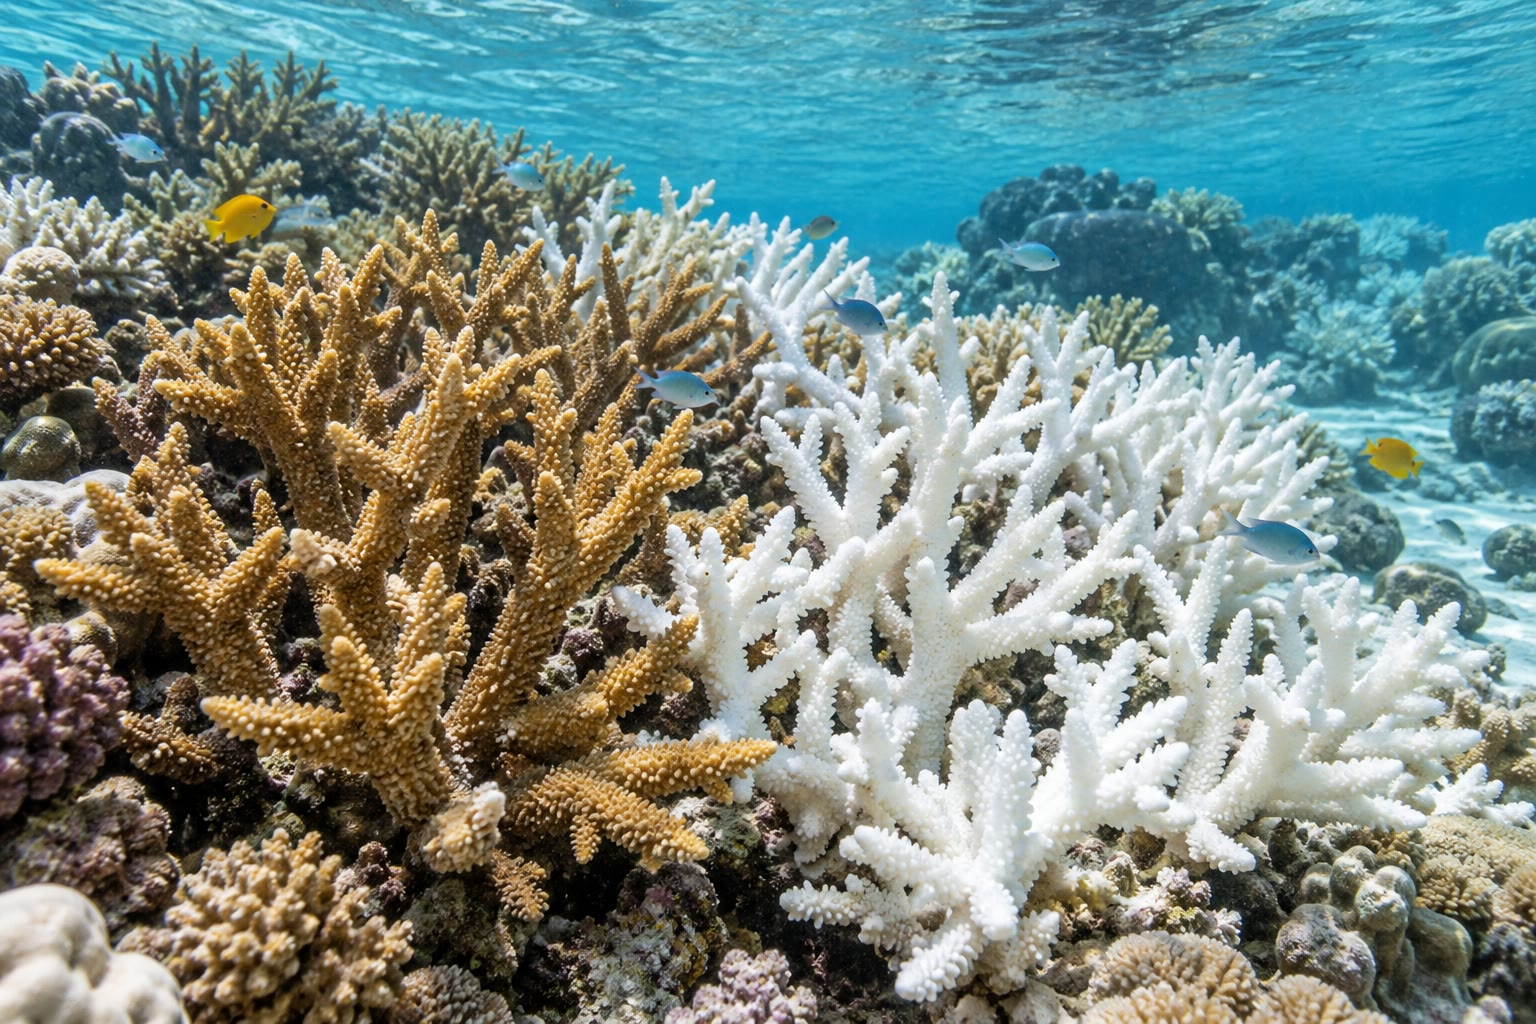
\includegraphics[width=0.44\linewidth]{images/book4/ai/b4-27-coral-bleaching.jpg}\hspace{0.04\linewidth}
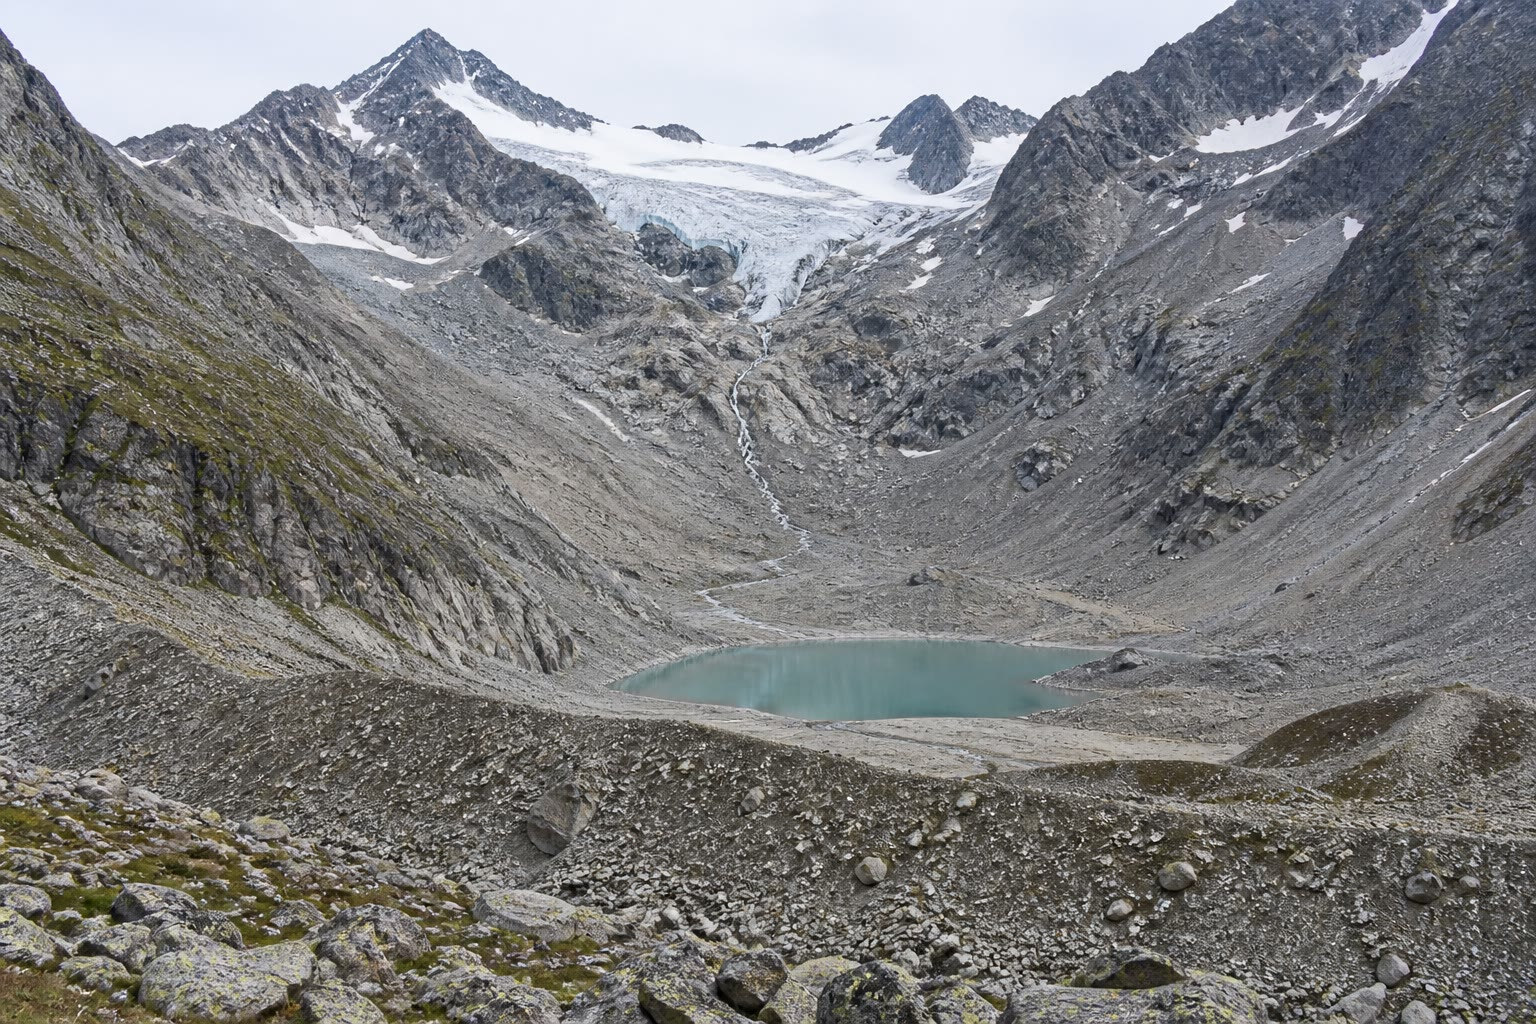
\includegraphics[width=0.44\linewidth]{images/book4/ai/b4-27-glacier-retreat.jpg}

{\small दो तापमापी। बाएँ: कोई विवर्णित रीफ़, जिसमें उस प्रवाल का सफ़ेद
कंकाल उस ऊतक से झाँकता है जो अपने शैवाल खो चुका है। दाएँ: कोई
घाटी-हिमनद जो अपनी घाटी में पीछे हट चुका है, और वहाँ नंगी चट्टान छोड़ गया है
जहाँ सदी भर पहले बर्फ़ खड़ी थी।}
\end{omfigure}

\section{बहीखाता: विलोपन और उसका आकलन}

\begin{theorem}[जाति--क्षेत्रफल संबंध और आवास-हानि की लागत]\label{thm:b2:global-change:sar}
\index{जाति--क्षेत्रफल संबंध}\index{विलोपन दर}\index{आवास-हानि}\index{विलोपन-ऋण}
किसी क्षेत्रफल $A$ में मिलती जातियों की संख्या उस क्षेत्रफल की किसी
घात की तरह बढ़ती है, $S = cA^{z}$, जिसमें द्वीपों तथा
आवास-खंडों के लिए $z \approx 0.25$ है (क्षेत्रफल दुगुना करना पाँचवाँ भाग और जातियाँ जोड़ता है; और
सौ गुना क्षेत्रफल, तीन गुनी)। यदि कोई आवास घटकर अपने विस्तार का
$1 - h$ अंश रह जाए, तो जितनी जातियाँ वह अंततः थाम सकता है वह संख्या
गिरकर मूल की $(1 - h)^{z}$ रह जाती है: यानी आधा आवास खोना
उसकी जातियों का \qty{16}{\%} लेता है, \qty{90}{\%} \qty{44}{\%} लेता है, और \qty{99}{\%}
\qty{68}{\%}। वह हानि तुरंत नहीं होती --- उस खंड में बचे हुए
कुछ समय तक टिकते हैं, यानी कोई \emph{विलोपन-ऋण} जो दशकों भर चुकाया जाता है
ज्यों-ज्यों छोटी समष्टियाँ \cref{ch:b2:population-genetics} के अपवाह तथा अंतःप्रजनन से
हार जाएँ --- और वही उस
आकलन का आधार है कि वर्तमान \omterm{thm:b2:global-change:sar}{विलोपन दर} जीवाश्म-अभिलेख की पृष्ठभूमि दर से
सौ से हज़ार गुना है: यानी प्रति वर्ष दस लाख में लगभग एक
जाति, जबकि कोई एक करोड़ में से प्रति वर्ष कई हज़ार
अब खोई जा रही हैं।
\end{theorem}
\begin{proof}
$S'/S = (A'/A)^{z} = (1 - h)^{z}$; और $z = 0.25$ के साथ, $0.5^{0.25} =
0.84$, $0.1^{0.25} = 0.56$, $0.01^{0.25} = 0.32$। वह संबंध
स्वयं आनुभविक है; और उसका घातांक द्वीपों पर उस संतुलन को दर्शाता है
जो नई जातियों के आप्रवास (जो उस द्वीप के भरने के साथ गिरता है)
और स्थानीयों के विलोपन (जो उनकी समष्टियों के क्षेत्रफल के साथ सिकुड़ने पर चढ़ता है) के बीच है,
यानी मैकआर्थर तथा विल्सन के सिद्धांत का वह साम्य।
\end{proof}
\begin{proof}[प्रमाण-सामग्री]
क्रकातोआ समूह के द्वीप, जो 1883 के उद्गार से निर्जीव हो गए थे,
पौधों, पक्षियों तथा कीटों ने ऐसे उत्तराधिकार में फिर बसाए
जो पचास वर्षों के भीतर उन जाति-संख्याओं तक पहुँचा
जो उनके क्षेत्रफलों से बताई गईं; और जिन मैंग्रोव-टापुओं को सिम्बरलॉफ़ तथा
विल्सन ने 1966 में फ़्लोरिडा में धूमित किया वे वर्ष भर के भीतर, भिन्न जातियों के साथ,
अपनी मूल जाति-संख्याओं पर लौट आए। ब्राज़ील का अटलांटिक
वन, जो घटकर अपने विस्तार का \qty{10}{\%} रह गया है, अपनी पक्षी-जातियों का वह अंश
खो चुका है या लगभग खो चुका है जो वह संबंध
बताता है; और विश्व संरक्षण संघ से आँके गए हर समूह में
एक चौथाई से एक तिहाई जातियाँ संकटग्रस्त हैं --- पक्षी
\qty{13}{\%}, स्तनी \qty{27}{\%}, उभयचर \qty{41}{\%}, प्रवाल
\qty{44}{\%} --- जिनमें आवास-हानि पहला कारण है, और शिकार,
\omterm{prop:b2:global-change:invasion}{आक्रामक जातियाँ}, प्रदूषण तथा, बढ़ते हुए, जलवायु बाक़ी।
\end{proof}

\begin{omfigure}
\begin{tikzpicture}
\begin{loglogaxis}[
  width=0.68\linewidth, height=5.4cm,
  axis x line=bottom, axis y line=left,
  xmin=1, xmax=100000, ymin=5, ymax=200,
  xlabel={द्वीप-क्षेत्रफल (\unit{km^2})}, ylabel={स्थल-पक्षियों की जातियाँ},
  xlabel style={font=\small, at={(axis description cs:0.5,-0.13)}, anchor=north},
  ylabel style={font=\small},
  tick label style={font=\small},
  clip=false,
]
\addplot[only marks, mark=*, mark size=2pt, omDef] coordinates {(1.5,9) (8,14) (35,22) (150,32) (400,37) (1200,52) (4000,70) (13000,92) (35000,125) (85000,160)};
\addplot[very thick, omThm, domain=1:100000, samples=2] {9*x^0.25};
\node[font=\scriptsize, omThm, anchor=north west, align=left] at (axis cs:2,120) {$S = 9A^{0.25}$: सौ गुना\\ अधिक क्षेत्रफल, तीन गुनी\\ जातियाँ};
\end{loglogaxis}
\end{tikzpicture}

{\small \omterm{thm:b2:global-change:sar}{जाति--क्षेत्रफल संबंध}, यहाँ किसी द्वीपसमूह के द्वीपों पर
स्थल-पक्षियों के लिए: यानी लघुगणकीय अक्षों पर $z = 0.25$ ढाल की कोई
सीधी रेखा। किसी आवास को दसवें भाग तक काटिए और वह, समय पाकर,
अपनी जातियों की आधी से थोड़ी ही अधिक रखेगा।}
\end{omfigure}

\begin{proposition}[आक्रमण, सेवाएँ, और क्या किया जा सकता है]\label{prop:b2:global-change:invasion}
\index{आक्रामक जाति}\index{पारितंत्र-सेवाएँ}\index{शमन}\index{शुद्ध शून्य}
जहाज़ों, विमानों तथा व्यापार ने हज़ारों जातियाँ उन
बाधाओं के पार चला दी हैं जो उन्हें अलग रखती थीं; अधिकांश जम नहीं पातीं, पर वे
कुछ जो पातीं --- ऑस्ट्रेलिया में ख़रगोश, ग्रेट लेक्स में ज़ेब्रा शंबुक,
वह भूरा वृक्ष-सर्प जिसने गुआम को उसके पक्षियों से ख़ाली कर दिया,
वह काइट्रिड कवक जिसने उभयचरों की नब्बे जातियाँ विलोपन तक पहुँचा दी हैं ---
अचल गति से आगे बढ़ती किसी अग्रिम-रेखा की तरह फैलती हैं, $c =
2\sqrt{rD}$, यानी दर $r$ से बढ़ती और विसरण गुणांक $D$ से
प्रकीर्ण होती किसी समष्टि के लिए (स्केलम का कस्तूरी-चूहा, जो 1905 में
प्राग के पास छोड़ा गया, यूरोप भर वर्ष भर में \qty{11}{km} फैला,
और उसकी परास-त्रिज्या समय में एक सीधी रेखा रही)। इस सबके सामने वह खड़ा है
जो वह जीवमंडल अपनी एक झंझटी जाति के लिए करता है:
तीन चौथाई फ़सलों का \omterm{def:b2:angiosperm-reproduction:pollination}{परागण}, जल-शोधन,
बाढ़-नियंत्रण, नाइट्रोजन का स्थिरीकरण तथा \omterm{def:b2:living-soil:soil}{मिट्टी} का बनना, मछलियाँ,
वनों तथा मिट्टियों में थमा कार्बन --- यानी \emph{पारितंत्र-सेवाएँ},
जिनका मूल्य, जहाँ उन पर कोई क़ीमत रखी जा सके, दुनिया के
आर्थिक उत्पाद से अधिक आँका जाता है। जो किया जा सकता है वह उन अंकों से निकलता है।
तापन तब रुकता है जब शुद्ध उत्सर्जन रुकें, उससे पहले नहीं:
\cref{ch:b2:biogeochemical-cycles} के \omterm{thm:b2:biogeochemical-cycles:box}{डिब्बा-प्रतिरूप}
\emph{\omterm{prop:b2:global-change:invasion}{शुद्ध शून्य}} का कोई और पाठ नहीं होने देते। ज़मीन सीमाओं के भीतर मदद कर सकती है ---
पुनर्वनीकरण तथा मिट्टियों से कुछ दशकों तक वर्ष भर में कार्बन का कोई
गीगाटन, जबकि जीवाश्म ईंधनों से दस --- और जातियों को चलने में
मदद दी जा सकती है, या उन्हें ऐसे बड़े तथा जुड़े रक्षित क्षेत्रों में रखा जा सकता है
कि वह \omterm{thm:b2:global-change:sar}{जाति--क्षेत्रफल संबंध} तथा छोटी समष्टियों का अपवाह
उन्हें ख़त्म न कर दें। वे औज़ार इसी पुस्तक के हैं: उस रक्षित क्षेत्र की
\omterm{def:b2:population-genetics:frequencies}{समष्टि आनुवंशिकी}, उस आक्रांता की होड़, उस फ़सल की
ऋतु-विज्ञान, उस \omterm{def:b2:living-soil:soil}{मिट्टी} का बजट।
\end{proposition}

\begin{example}[तीन भविष्य]\label{ex:b2:global-change:scenarios}
वर्ष भर में \qty{10}{GtC} पर 2100 तक थामे गए उत्सर्जन पहले ही उत्सर्जित
\qty{700}{} में \qty{800}{GtC} जोड़ देते हैं: यानी सदी के अंत तक $1.65\times 1.5 =
\qty{2.5}{\celsius}$ और अब भी चढ़ता। 2070 तक शून्य तक गिरते उत्सर्जन
लगभग \qty{250}{GtC} जोड़ते हैं: \qty{1.6}{\celsius},
और फिर समतल। पहले उत्सर्जन दुगुने करना, जैसा सदी के आरंभिक
दशकों ने किया, \qty{4}{\celsius} या उससे अधिक देता है। समशीतोष्ण
कटिबंध के परास पहली स्थिति में आज के परे \qty{200}{km} चलते हैं
और दूसरी में \qty{60}{km}; वसंत पच्चीस
दिन पहले आता है, या छह; सतही pH $7.8$ तक पहुँचता है, या
$8.0$ के पास रहता है; और वे विलोपन-आकलन, जो आवास तथा
तापन दोनों पर निर्भर हैं, जातियों के दसवें भाग से एक तिहाई तक जाते हैं।
उन भविष्यों के बीच का अंतर किसी एक वक्र के नीचे का संचयी क्षेत्रफल है,
जो अभी न लिए गए निर्णयों का योग है।
\end{example}

\section{अभ्यास}

\begin{exercise}[$\star$]\label{exo:b2:global-change:1}
तापन तथा \omterm{prop:b2:global-change:tcre}{संचयी उत्सर्जनों} के बीच का संबंध बताइए, और
700, 1000 तथा \qty{2000}{GtC} के \omterm{prop:b2:global-change:tcre}{संचयी उत्सर्जनों} के लिए
तापन निकालिए।
\end{exercise}

\begin{exercise}[$\star$]\label{exo:b2:global-change:2}
अंश-दिन तथा \omterm{thm:b2:global-change:phenology}{ऋतु-वैज्ञानिक बेमेल} की परिभाषा दीजिए, और उदाहरण के रूप में
वह मक्खीमार।
\end{exercise}

\begin{exercise}[$\star$]\label{exo:b2:global-change:3}
समताप-रेखाएँ प्रति अंश तापन पर ऊपर की ओर तथा ध्रुव की ओर कितनी दूर चलती हैं,
और कोई पर्वत-शीर्ष की जाति पीछे क्यों नहीं चल सकती?
\end{exercise}

\begin{exercise}[$\star$]\label{exo:b2:global-change:4}
तीन वाक्यों में समझाइए कि समुद्र में \ensuremath{\mathrm{CO_2}} जोड़ना
उसका pH तथा उसका कार्बोनेट क्यों गिराता है, और किन जीवों को चोट लगती है।
\end{exercise}

\begin{exercise}[$\star\star$]\label{exo:b2:global-change:5}
$\lambda = \qty{1.65}{\celsius}$ प्रति \qty{1000}{GtC} तथा पहले ही
उत्सर्जित \qty{700}{GtC} के साथ \qty{1.5}{\celsius} के लिए और
\qty{2}{\celsius} के लिए बचा \omterm{prop:b2:global-change:tcre}{कार्बन बजट} निकालिए; और दोनों को
\qty{10}{GtC/yr} पर वर्षों में बदलिए।
\end{exercise}

\begin{exercise}[$\star\star$]\label{exo:b2:global-change:6}
वसंत \qty{5}{\celsius} के किसी आधार से प्रति दिन $b = \qty{0.12}{\celsius}$
से गरम होता है; किसी पतंगे को $K = 150$ अंश-दिन चाहिए।
आधार पार करने से निर्गमन तक दिन, और \qty{1.5}{\celsius} के किसी
तापन के लिए वह जल्दी आना निकालिए।
\end{exercise}

\begin{exercise}[$\star\star$]\label{exo:b2:global-change:7}
किसी पौधे का परास \qty{1800}{m} ऊँचे किसी पर्वत पर, जिसका क्षेत्रफल ऊँचाई के
हर \qty{300}{m} पर आधा हो जाता है, \qtyrange{800}{1400}{m} फैला है।
\qty{3}{\celsius} तापन के बाद वह पट्टी कहाँ है और उसने कितना
क्षेत्रफल खोया है? \qty{5}{\celsius} के बाद?
\end{exercise}

\begin{exercise}[$\star\star$]\label{exo:b2:global-change:8}
560, 800 तथा \qty{1000}{ppm} पर सतही pH और हाइड्रोजन-आयन
सांद्रता में चढ़ाई निकालिए, $\mathrm{pH} = 8.2 -
0.9\log_{10}(p/280)$ से।
\end{exercise}

\begin{exercise}[$\star\star$]\label{exo:b2:global-change:9}
$z = 0.25$ के साथ, किसी आवास का \qty{70}{\%}, \qty{95}{\%} तथा
\qty{99.9}{\%} नष्ट होने पर जातियों का कौन-सा अंश अंततः खोता है?
तुरंत हानि छोटी क्यों है?
\end{exercise}

\begin{exercise}[$\star\star\star$]\label{exo:b2:global-change:10}
कोई आक्रांता प्रति वर्ष $r = 0.7$ से बढ़ता है और $D =
\qty{20}{km^2/yr}$ से प्रकीर्ण होता है। उसकी अग्रिम-गति और \qty{1000}{km}
चौड़े किसी देश को पार करने का काल निकालिए। उस गति को क्या आधा करता है: $r$ आधा करना
या $D$ आधा करना?
\end{exercise}

\begin{exercise}[$\star\star\star$]\label{exo:b2:global-change:11}
पृष्ठभूमि \omterm{thm:b2:global-change:sar}{विलोपन दर} प्रति दस लाख जाति-वर्ष 1 है और
80 लाख जातियाँ हैं। पृष्ठभूमि पर, और पृष्ठभूमि से 1000 गुना पर, प्रति
वर्ष तथा प्रति सदी प्रत्याशित विलोपन निकालिए।
पिछली सदी के दस हज़ार प्रलेखित विलोपनों से तुलना कीजिए और उस विसंगति
पर टिप्पणी कीजिए।
\end{exercise}

\begin{exercise}[$\star\star\star$]\label{exo:b2:global-change:12}
``तापन तब रुकता है जब शुद्ध उत्सर्जन रुकें।'' वायुमंडल के
\omterm{thm:b2:biogeochemical-cycles:box}{डिब्बा-प्रतिरूप} और \omterm{prop:b2:global-change:tcre}{संचयी उत्सर्जनों} के प्रति तापन की समानुपातिता से
इसे सिद्ध कीजिए, और कहिए कि उस तर्क में से क्या ग़ायब है।
\end{exercise}

\section{समस्या: 2100 में जीवमंडल}

\begin{problem}[{सप्तांत समस्या --- दो उत्सर्जन-पथ 2100 तक
ले जाए गए: हर एक का तापन, वह जो वसंत बनाता है, उसकी समताप-रेखाएँ
जितनी दूरी चलती हैं, वह जो अम्ल समुद्र में डालता है और वे जातियाँ जो वह
किसी वन को पड़ती हैं, और अंत उन दो तापनों, उन दो pH मानों
तथा खोई जातियों के अंश पर}]
\label{pb:b2:global-change:1}
आँकड़े। $\lambda = \qty{1.65}{\celsius}$ प्रति \qty{1000}{GtC};
2020 तक उत्सर्जित \qty{700}{GtC} (तापन \qty{1.2}{\celsius})। पथ
A: 2100 तक अचल \qty{10}{GtC/yr}। पथ B: 2070 में रैखिक रूप से
शून्य तक गिरता। वसंत \qty{5}{\celsius} के किसी आधार से ऊपर प्रति दिन
$b = \qty{0.1}{\celsius}$ से गरम होता है; किसी वृक्ष को पत्ती निकालने को $K = 200$
अंश-दिन चाहिए, और कोई प्रवासी पक्षी किसी नियत तिथि पर पहुँचता है,
यानी 2020 में उस वृक्ष के पत्ती निकालने के 20 दिन बाद। \omterm{prop:b2:global-change:range}{ह्रास दर}
\qty{6.5}{\celsius/km}; अक्षांशी प्रवणता \qty{100}{km} पर
\qty{0.65}{\celsius}। महासागर: $\mathrm{pH} = 8.2 - 0.9\log_{10}(p/280)$;
2100 में \ensuremath{\mathrm{CO_2}}: पथ A पर \qty{600}{ppm}, पथ B पर \qty{420}{ppm}।
400 वृक्ष-जातियों तथा $z = 0.25$ वाला \qty{e5}{km^2} का कोई वन-क्षेत्र
2100 तक पथ A पर सफ़ाई को अपने क्षेत्रफल का \qty{60}{\%} और
पथ B पर \qty{20}{\%} खो देता है।

\medskip
\noindent\textbf{भाग I --- तापन।}
\begin{enumerate}
  \item हर पथ पर 2100 में \omterm{prop:b2:global-change:tcre}{संचयी उत्सर्जन} निकालिए।
  \item हर पथ पर 2100 में तापन निकालिए।
  \item हर एक पर 2050 में तापन निकालिए।
  \item पथ A पर प्रति दशक तापन-दर क्या है? देखी गई
        \qty{0.2}{\celsius} प्रति दशक से तुलना कीजिए।
  \item पथ B पर, क्या वह तापन 2070 में रुक जाता है? उस
        समानुपातिता के अनुसार क्यों?
  \item कौन-सा \omterm{prop:b2:global-change:tcre}{संचयी उत्सर्जन} \qty{2}{\celsius} के अनुरूप है,
        और पथ A उसे किस वर्ष पार करता है?
\end{enumerate}

\medskip
\noindent\textbf{भाग II --- वसंत।}
\begin{enumerate}[resume]
  \item 2020 में आधार पार करने से पत्ती निकलने तक दिन निकालिए।
  \item हर पथ पर 2100 में, 2020 के सापेक्ष, पत्ती निकलने का जल्दी आना
        निकालिए (तापन 2020 के सापेक्ष)।
  \item उस पक्षी की पहुँचने की तिथि नहीं बदलती। 2100 में हर पथ पर
        पत्ती निकलने तथा पहुँचने के बीच का अंतर निकालिए।
  \item जिन इल्लियों को वह पक्षी चाहता है वे पत्ती निकलने के 15 दिन बाद शिखर पाती हैं
        और 10 दिन चलती हैं। किस पथ पर वह पक्षी उन्हें अब भी पाता है?
  \item मान लीजिए इसके बजाय वह पक्षी प्रति अंश \qty{3}{d} जल्दी आता
        है। पथ A पर वह अंतर फिर से निकालिए।
  \item एक वाक्य में बताइए कि उस पक्षी को वह बेमेल क्यों संकट में डालता है, स्वयं वह तापन नहीं।
\end{enumerate}

\medskip
\noindent\textbf{भाग III --- परास।}
\begin{enumerate}[resume]
  \item हर पथ पर, 2020 के सापेक्ष, समताप-रेखाओं का
        ऊँचाई-संबंधी तथा अक्षांशी विस्थापन निकालिए।
  \item कोई वृक्ष-जाति वर्ष भर में \qty{100}{m} प्रकीर्ण होती है। क्या वह पथ A पर
        उन समताप-रेखाओं के पीछे ध्रुव की ओर चल सकती है? पथ B पर?
  \item कोई जाति \qty{2000}{m} के किसी पर्वत पर \qtyrange{1500}{1800}{m}
        घेरती है। पथ A पर 2100 में उसकी पट्टी कहाँ बैठती है,
        और क्या होता है?
  \item उस पर्वत का क्षेत्रफल हर \qty{300}{m} पर आधा हो जाता है। पथ B पर उस
        जाति द्वारा खोया गया क्षेत्रफल-गुणक निकालिए।
  \item कोई समुद्री मछली प्रति दशक \qty{30}{km} से समताप-रेखाओं के पीछे चलती है।
        क्या वह पथ A पर काफ़ी है?
  \item समझाइए कि किसी परास का निचला किनारा वहाँ भी क्यों पीछे हटता है जहाँ
        वह जाति उस गरमी को सह सकती हो।
\end{enumerate}

\medskip
\noindent\textbf{भाग IV --- समुद्र और वन।}
\begin{enumerate}[resume]
  \item हर पथ पर 2100 में सतही pH, और 1750 से हाइड्रोजन-आयन
        सांद्रता में चढ़ाई निकालिए।
  \item उष्णकटिबंधीय सतह की \omterm{thm:b2:global-change:acid}{संतृप्ति अवस्था} $\Omega$ 1750 में
        4 थी और $[\ensuremath{\mathrm{H^{+}}}]^{-1}$ की तरह गिरती है। हर पथ पर 2100 में उसे
        निकालिए और कहिए कि प्रवाल के लिए उसका क्या अर्थ है।
  \item हर पथ पर वह वन-क्षेत्र अंततः जितनी वृक्ष-जातियाँ थाम सकता है
        वह संख्या, और खोई गई संख्या निकालिए।
  \item तापन और हानियाँ जोड़ता है: मान लीजिए 2020 से ऊपर हर अंश
        बची हुई जातियों का और \qty{5}{\%} हटा देता है। हर पथ पर
        बची जातियाँ फिर से निकालिए।
  \item हर पथ पर उन 400 जातियों का खोया अंश दीजिए।
  \item उन दोनों कारणों में से, सफ़ाई या तापन, हर पथ पर कौन हावी है?
  \item परिणाम बताइए: हर पथ पर 2100 में तापन, pH और खोई
        वृक्ष-जातियों का अंश।
\end{enumerate}
\end{problem}
